\fontsize{13}{14}\selectfont
\section{PROCEDURE}

\subsection{Load data}

\begin{lstlisting}[style=StyleCode, language=MATLAB]
	% Clear the workspace
	clear;
	% Load the user_movies.mat file
	load('users_movies.mat', 'movies', 'users_movies', 'users_movies_sort', 'index_small', 'trial_user')
\end{lstlisting}

First, we load the data from the file “\texttt{users\_movies.mat}” using the “\texttt{load}” command. "\texttt{load}" helps us to load actual data stored in those variables shown below while "\texttt{clear}" is used to clear all variables in MATLAB workspace to ensure that no old data interferes. The matrix “\texttt{users\_movies}” should have dimensions $6040 \times 3952$, with integer values ranging from 0 to 5. A rating of 1 represents “strongly dislike”, while 5 represents “strongly like”. A rating of 0 indicates that the user did not rate the movie. The array “movies” contains the titles of all the movies. Moreover, the matrix “users movies sort” is a subset of “\texttt{users\_movies}”, containing ratings for the 20 most popular movies.

\begin{center}
	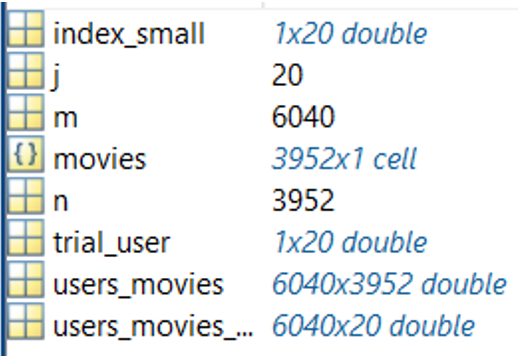
\includegraphics[width=.3\linewidth]{sections/pic/section3/1.png}
\end{center}

Also, the indexes of these popular movies are stored in the array “\texttt{index\_small}”. Finally, the vector “\texttt{trial\_user}” contains ratings of these popular movies by another user who is not part of the database. It is recommended to view all variables and their dimensions using the “Workspace” window in the MATLAB environment.

\subsection{Print the titles}

The figure below shows the 20 most popular movies:

\begin{lstlisting}[style=StyleResult]
	The rating is determined based on the 20 most popular movies:
	1. E.T. the Extra-Terrestrial (1982)
	2. Star Wars Episode IV - A New Hope (1977)
	3. Star Wars Episode V - The Empire Strikes Back (1980)
	4. Star Wars Episode VI - Return of the Jedi (1983)
	5. Jurassic Park (1993)
	6. Saving Private Ryan (1998)
	7. Terminator 2: Judgment Day (1991)
	8. The Matrix (1999)
	9. Back to the Future (1985)
	10. The Silence of the Lambs (1991)
	11. Star Wars Episode I - The Phantom Menace (1999)
	12. Raiders of the Lost Ark (1981)
	13. Fargo (1996)
	14. The Sixth Sense (1999)
	15. Braveheart (1995)
	16. Shakespeare in Love (1998)
	17. The Princess Bride (1987)
	18. Schindler's List (1993)
	19. The Shawshank Redemption (1994)
	20. Groundhog Day (1993)
\end{lstlisting}

The code below is use to print top 20 most popular movies.

\begin{lstlisting}[style=StyleCode, language=MATLAB]
	% Get the dimensions
	[m, n] = size(users_movies);
	
	% Print a header indicating the movies to be listed
	fprintf('The rating is determined based on the %d most popular movies: \n', length(index_small))
	
	% Loop through of the popular movies
	for j = 1:length(index_small)
		% print the movies title correponding to the current index
		fprintf('%d. %s \n', j, movies(index_small(j)));
	end
	fprintf('\n);
\end{lstlisting}

The "\texttt{fprintf()}" function is a versatile tool used to display formatted text directly in the Command Window. When constructing the output string, special format specifiers are used to indicate how different types of data should be displayed. For instance, "\texttt{\%d}" serves as a placeholder that allows for the printing of an integer value. To control the layout of the output, the newline character, represented as "\texttt{\textbackslash n}", is used to move the cursor to the beginning of the next line, effectively adding a line break.

Generally, "\texttt{length(index\_small)}" is used to determine the total number of elements within an array named "\texttt{index\_small}". This numerical result can then be incorporated into a formatted string using "\texttt{fprintf()}" and the "\texttt{\%d}" specifier to display this count.

Loops are fundamental for repetitive tasks, and the "\texttt{for}" loop is commonly used to execute a block of code multiple times. Within such a loop, “\texttt{fprintf()}” can be employed again to print details for each iteration.

For example, the format string "\texttt{\%d. \%s \textbackslash n}" instructs the program to print an integer (using \texttt{\%d}), followed by a period and a space, then a string of characters (using \texttt{\%s}), and finally, to add a new blank line (\texttt{\textbackslash n}). In short:

\begin{itemize}[label=-]
	\item \textbf{\texttt{\%d}:} Prints the index interger.
	\item \textbf{\texttt{\%s}:} Prints the title movies.
	\item \textbf{\texttt{\textbackslash n}:} Adds new blank line.
\end{itemize}

This is useful for creating numbered lists, such as displaying an index number alongside a movie title. To further improve the visual separation and readability of the output, an additional "\texttt{{fprintf('\textbackslash n')}}" can be used to print an extra blank line, creating better spacing in the Command Window.

\subsection{Select people}

The following code selects people who rated all of the 20 movies under consideration:

\begin{lstlisting}[style=StyleCode, language=MATLAB]
	% Select the users to compare to 
	[m1, n1] = size(users_movies_sort);
	rating = [];
	for j = 1:m1
		if prod(users_movies_sort(j, :)) ~= 0
			rating = [rating; users_movies_sort(j, :)];
		end;
	end;
\end{lstlisting}

\textbf{Explain:}

Initially, the code determines the dimensions of a matrix named "\texttt{users\_movies\_sort}" by using the "\texttt{size()}" function. This function call assigns the number of rows (representing users) to the variable m1 and the number of columns (representing movies) to \texttt{n1}. Following this, an empty matrix called ratings is created, which will be used to store selected user data:

\begin{itemize}[label=-]
	\item \texttt{[m1, n1] = size(users\_movies\_sort)}: Measure the size of the users\_movies\_sort matrix. m1 is the number of users (rows), n1 is the number of movies (columns).
	\item \texttt{ratings = []}: Create an empty matrix called ratings.
\end{itemize}

The core of this code segment is a for loop that iterates through each user, from the first user (index 1) up to m1 (the total number of users). Inside this loop, a conditional check is performed using an if statement. This condition evaluates the product of all ratings for the current user \texttt{j} (accessed via \texttt{users\_movies\_sort(j, :)}). If this product is not equal to zero (\texttt{\textasciitilde = 0}), it implies that the user has provided a rating for every movie (assuming no rating is represented by a zero). When this condition is true, that user's entire row of ratings from \texttt{users\_movies\_sort} is appended to the ratings matrix.

\begin{lstlisting}[language=MATLAB]
	for j = 1:m1                         
		if prod(users_movies_sort(j, :)) ~= 0  
		ratings = [ratings; users_movies_sort(j, :)];  
	end;
\end{lstlisting}

The whole point of this is to sort out users that rate all the film they watched and add their ratings to a set.

\textbf{Question 1: What does the command \texttt{ratings=[]} do?}

This initializes an empty array named ratings that ratings start with no elements. This setup is commonly used to collect or build up data in subsequent operations, specially 
within loops. The code then iterates over \texttt{users\_movies\_sort} array and adds rows to ratings for users who have rated all the movies they watched.

The below table shows a part of the result of ratings after the execution of the source code:

\begin{figure}[H]
	\centering
	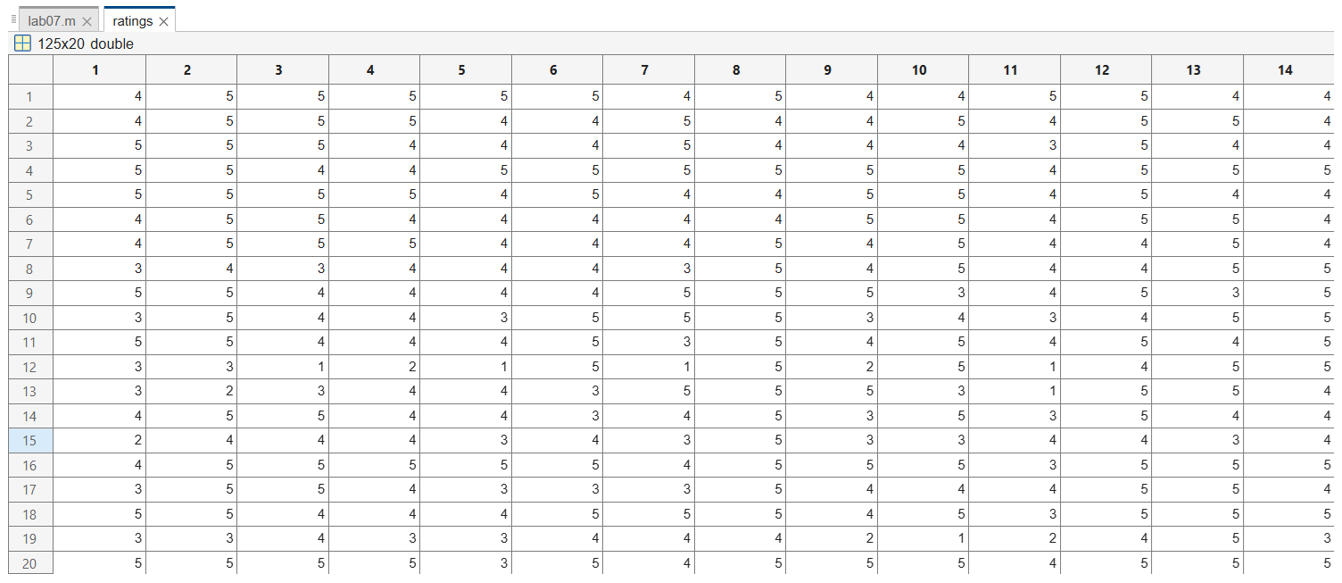
\includegraphics[width=.9\linewidth]{sections/pic/section3/2.png}
\end{figure}

\subsection{Find the Euclidean distance}

The following code calculates the Euclidean distance:

\begin{lstlisting}[style=StyleCode, language=MATLAB]
	% Find the Euclidean distance
	[m2, n2] = size(ratings);
	for i = 1:m2
		eucl(i) = norm(ratings(i,:)-trial_users);
	end;
\end{lstlisting}

In this part, we would calculate the Euclidean distance to measure the similarity between a specific “\texttt{trial\_user}” and every other user within the ratings dataset.

Where:

\begin{itemize}[label=-]
	\item \texttt{ratings(i, :)}: is the vector of movie ratings for i-th user.
	\item \texttt{trial\_user}: is the vector of movie ratings for the trial user (the user whose similarities we want to find).
\end{itemize}

The first step in the comparison involves element-wise subtraction, \texttt{ratings(i,:) - trial\_user}.

\begin{itemize}[label=-]
	\item \texttt{ratings(i,:)-trial\_users}: computes the difference between the i-th user's ratings and the trial user's ratings for each movie. 
\end{itemize}

Subsequently, the “\texttt{norm()}” function is applied to this difference vector specifically,

\begin{itemize}[label=-]
	\item \texttt{norm(ratings(i,:)-trial\_users)}: calculates the Euclidean distance between these two vectors.
\end{itemize}

The resulting distance for each comparison is stored in “\texttt{eucl(i)}”,

\begin{itemize}[label=-]
	\item \texttt{eucl(i)}: represents the Euclidean distance between the \texttt{trial\_user} and the i-th user in the ratings array (or matrix). The smaller the value of \texttt{eucl(i)}, the more similar the i-th user's ratings are to the trial user's ratings, this means that the i-th user has comparable tastes in movies to the \texttt{trial\_user}.
\end{itemize}

Moreover, the eucl vector contains a series of Euclidean distances, each representing the similarity between a trial user and other users in a dataset. A portion of this vector is displayed in the table, showing various distance values calculated:

\begin{figure}[H]
	\centering
	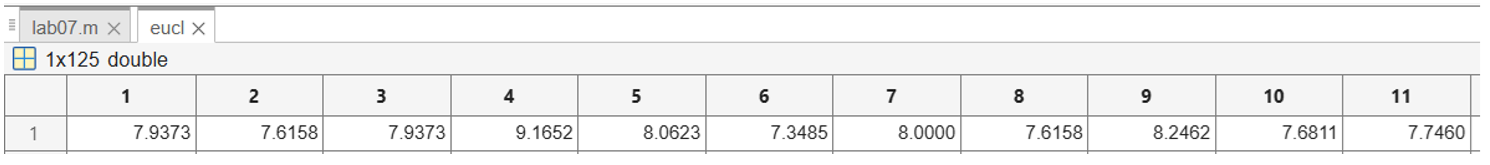
\includegraphics[width=\linewidth]{sections/pic/section3/3.png}
\end{figure}

The command “\texttt{[smallest\_number, position] = min(eucl);}” processes the eucl vector to find its minimum value and the index at which this minimum occurs. The minimum value is stored in the variable "smallest\_number", while its corresponding index (or position within the vector) is stored in the variable position. Following this computation, the code uses \texttt{disp()} commands to output these findings:

\begin{lstlisting}[style=StyleCode, language=MATLAB]
	% Find the smallest Euclidean distance
	[smallest\_number, position] = min(eucl);
	disp(['Smallest Eucl: ', num2str(smallest_number)]);
	disp(['Position: ', num2str(position)]);
\end{lstlisting}

Upon running the code, the results indicate that the smallest Euclidean distance found is $5.6569$, and this value corresponds to position $14$ in the eucl vector. This means that the 14th person in the ratings data has rating patterns most closely matching the trial user, with a calculated Euclidean distance of $5.6569$, which is shown in the figure below:

\begin{lstlisting}[style=StyleResult]
	Smallest Eucl: 5.6569
	Position: 14
\end{lstlisting}

\subsection{Find the Pearson correlation coefficient}

Initially, we create a zero vector to save the coefficient. This vector will eventually store the calculated Pearson correlation coefficient for each user in the ratings matrix when compared against the \texttt{trial\_user}. Concurrently, the trial\_user's rating vector is reshaped into a column vector using \texttt{trial\_user(:);} to ensure it is correctly oriented for the subsequent matrix operations, as shown in the figure below.
	
	\begin{lstlisting}[style=StyleCode, language=MATLAB]
		% Compute the Pearson correlation coefficient
		pearson = zeros(size(ratings, 1), 1);
		trial_user = trial_user(:);
		
		% Compute correlation along the ratings vectors
		for i = 1:size(ratings, 1)
		current_rating = ratings(i, :);
		
		% Compute mean
		trial_user_mean = mean(trial_user);
		current_ratings_mean = mean(current_rating);
		
		% Subtract with the mean
		trial_user_centered = trial_user - trial_user_mean;
		current_ratings_centered = current_rating - current_ratings_mean;
		
		pearson_numerator = sum(trial_user_centered .* current_ratings_centered);
		pearson_denominator = sqrt(sum(trial_user_centered .^ 2) .* sum(current_ratings_centered .^ 2));
		
		if pearson_denominator == 0
		comr = pearson_numerator / pearson_denominator;
		else
		comr = 0;
		end
		
		pearson(i) = comr;
		end
		
		% Find the highest Pearson correlation coefficient
		[max_pearson, pearson_index] = max(pearson);
		disp(['Highest Pearson correlation coefficient: ', num2str(max_pearson)]);
		disp(['Position: ', num2str(pearson_index)]);
	\end{lstlisting}
	
\begin{itemize}[label=-]
	\item \texttt{pearson = zeros(size(ratings, 1), 1);}: The line initializes a column vector ‘pearson’ of zeros, with a length equal to the number of users (rows) in the ‘ratings’ matrix. This will store the Pearson correlation coefficients for each user compared to the trial user.
	\item \texttt{trial\_user = trial\_user(:)';}:'\texttt{trial\_user(:)}' reshapes the ‘\texttt{trial\_user}’ vector into a column vector. ‘'’ (transpose) converts it back into a row vector.
\end{itemize}

This ensures that ‘\texttt{trial\_user}’ is properly oriented for matrix operations that follow.

We then create a loop to traverse along the rows of rating vectors which is the rating of each user in database to compute the Pearson correlation coefficient with the trial user rating by the formula below:

\[ r = \dfrac{\sum (x_{i} - \bar{x})(y_{i} - \bar{y})}{\sqrt{\sum (x_{i} - \bar{x})^{2} \sum (y_{i} - \bar{y})^{2}}} \]

The process to compute the Pearson correlation coefficient:

\begin{enumerate}[label=Step \arabic*: ]
	\item Compute the mean of 2 sets:
		\[ \bar{x} = \dfrac{\sum x_{i}}{n x} ; \bar{y} = \dfrac{\sum y_{i}}{n y} \]
	\item Compute the subtracted vectors from 2 sets by their means:
		\begin{itemize}[label=-]
			\item For set '$x$', the centered vector $x_{s}$ would have elements: $ x_{si} = x_{i} - \bar{x} $.
			\item For set '$y$', the centered vector $y_{s}$ would have elements: $y_{si} = y_{i} - \bar{y}$.
		\end{itemize}
	\item Compute the numeration: $\sum(x_{si} \cdot y_{si})$.
	\[ \sqrt{\sum x_{si}^{2}} \cdot \sqrt{\sum y_{si}^{2}} \]
	\item Compute the denominator.
	\item Divide the numerator from step 3 with the denominator in step 4.
\end{enumerate}

\begin{lstlisting}[style=StyleCode, language=MATLAB]
	for i = 1:size(ratings, 1)
	current_rating = ratings(i, :);
\end{lstlisting}

This ‘\texttt{for}’ loop iterates over each user's ratings in the ‘\texttt{ratings}’ matrix. ‘\texttt{current\_rating}’ stores the ratings of the i-th user (row) for all items. 

\begin{lstlisting}[style=StyleCode, language=MATLAB]
	trial_user_mean = mean(trial_user); 
	current_ratings_mean = mean(current_rating); 
\end{lstlisting}

‘\texttt{trial\_user\_mean}’ calculates the \texttt{mean} (average) rating of the trial user. ‘\texttt{current\_ratings\_mean}’ calculates the mean rating of the i-th user. 
These means are used to center the ratings by subtracting the mean from each rating.

\begin{lstlisting}[style=StyleCode, language=MATLAB]
	trial_user_centered = trial_user - trial_user_mean;
	current_ratings_centered = current_rating - current_ratings_mean;
\end{lstlisting}

These lines subtract the mean rating from each user's individual ratings, centering the data. ‘\texttt{trial\_user\_centered}’ contains the trial user's centered ratings.
‘\texttt{current\_ratings\_centered}’ contains the centered ratings of the i-th user.
Centering helps in comparing the patterns in the ratings, ignoring the absolute values.

\begin{lstlisting}[style=StyleCode, language=MATLAB]
	pearson_numerator = sum(trial_user_centered.* current_ratings_centered);
\end{lstlisting}

This calculates the numerator of the Pearson correlation coefficient formula. ‘\texttt{.*}’ performs element-wise multiplication of the centered ratings.
‘\texttt{sum}’ adds up the results of these multiplications.

\begin{lstlisting}[style=StyleCode, language=MATLAB]
	pearson_denominator = sqrt(sum(trial_user_centered .^2) .* sum(current_ratings_centered .^2));
\end{lstlisting}

This calculates the denominator of the Pearson correlation coefficient formula.
‘\texttt{.\^2}’ squares each element in the centered rating vectors.
‘\texttt{sum}’ adds up these squared values. ‘\texttt{sqrt}’ takes the square root of the product of these sums.

\begin{lstlisting}[style=StyleCode, language=MATLAB]
	if pearson_denominator ~= 0 
		corr = pearson_numerator / pearson_denominator; 
	else 
		corr = 0; 
	end; 
\end{lstlisting}

This conditional statement checks if the denominator is non-zero to avoid division by zero. 

If the denominator is non-zero, ‘\texttt{corr}’ is calculated as the Pearson correlation coefficient. 

If the denominator is zero (which can happen if one of the users has constant ratings), ‘\texttt{corr}’ is set to 0.

\subsection{Find the highest Pearson coefficient}

\begin{lstlisting}[style=StyleCode, language=MATLAB]
	% Compute the Pearson correlation coefficient
	pearson = zeros(size(ratings, 1), 1);
	trial_user = trial_user(:)';
	
	% Compute correlation along the ratings vectors
	for i = 1:size(ratings,1)
		current_rating = ratings(i, :);
		
		% Compute mean 
		trial_user_mean = mean(trial_user);
		current_rating_mean = mean(current_rating);
		
		% Subtract the mean
		trial_user_centered = trial_user - trial_user_mean;
		current_rating_centered = current_rating - current_rating_mean;
		
		% Compute numerator and denominator
		pearson_numerator = sum(trial_user_centered .* current_rating_centered);
		pearson_denominator = sqrt(sum(trial_user_centered .^ 2) * sum(current_rating_centered .^ 2));
		
		% Avoid division by zero
		if pearson_denominator ~= 0
			corr = pearson_numerator / pearson_denominator;
		else
			corr = 0;
		end
		
		pearson(i) = corr;
	end;
	
	% Find the highest Pearson correlation coefficient
	[max_pearson, pearson_index] = max(pearson);
	disp(['Highest Pearson correlation coefficient: ', num2str(max_pearson)]);
	disp(['Position: ', num2str(pearson_index)]);
\end{lstlisting}

\begin{itemize}[label = -]
	\item \texttt{pearson(i) = corr}: The Pearson correlation value '\texttt{corr}' is stored at position '\texttt{i}' in the '\texttt{pearson}' array for each user analyzed in the loop. This process continues until all users have been evaluated for their similarity to the trial user.
	\item \texttt{[max\_pearson, pearson\_index] = max(pearson);}: This function locates both the maximum Pearson correlation value in the array and identifies its position. 
	The '\texttt{max\_pearson}' variable holds the highest correlation coefficient (indicating the user with the most similar rating patterns). While '\texttt{pearson\_index}' records this user's position within the '\texttt{ratings}' matrix.
	\item \texttt{disp(['Highest Pearson correlation coefficient: ', num2str(max\_pearson)]);} and \texttt{disp(['Position: ', num2str(pearson\_index)]);}: These commands display the highest calculated correlation coefficient and the position of the most similar user. ‘\texttt{num2str}’ converts the numeric values to strings for display purposes. ‘\texttt{disp}’ prints out the text and the computed values.
\end{itemize}

After execution, the analysis shows:

\begin{lstlisting}[style=StyleResult]
	Highest Pearson correlation coefficient: 0.62896
	Position: 88
\end{lstlisting}

\subsection{Compare the elements}

This section examines the difference between users identified as similar through two distinct methods: Euclidean distance and Pearson correlation.

\begin{lstlisting}[style=StyleCode, language=MATLAB]
	% Compare the elements of the vectors DistIndex, PearsonIndex
	% Use the position of the smallest Euclidean distance
	closest_user_Dist = position;
	
	% Use the index of the highest Pearson correlation coefficient
	closest_user_Pearson = pearson_index;
	
	% Compare if the closest user by Euclidean distance is the same as the closest user by Pearson correlation
	if closest_user_Dist == closest_user_Pearson
		disp(['The closest user based on Euclidean distance is the same as the closest user based on Pearson correlation.']);
	else
		disp(['The closest user based on Euclidean distance is different from the closest user baesd on Pearson correlation.']);
	end
	
	% Display the top 5 users for both distance and Pearson correlatin for comparison
	fprintf('\nTop closeest users baesed on Euclidean distance:\n');
	if length(position) >= 5
		disp(position(1:5)');
	else 
		disp(position');
	end
	
	fprintf('Top closest users based on Pearson correlation:\n');
	if length(pearson_index) >= 5
		disp(pearson_index(1:5)');
	else
		disp(pearson_index');
	end
\end{lstlisting}

The DistIndex vector identifies users with preferences closest to the trial user based on the Euclidean distance metric. This method calculates the "straight-line" distance between the trial user’s ratings and each other user’s ratings.

The PearsonIndex vector identifies users with preferences closest to the trial user based on the Pearson correlation coefficient. This method measures the linear correlation between the trial user’s ratings and each other user’s ratings, accounting for how well the users' preferences align in terms of direction (both users like/dislike similar movies)

\begin{lstlisting}[style=StyleResult]
	The closest user based on Euclidean distance is different from the closest user baesd on Pearson correlation.
	Top closeest users baesed on Euclidean distance:
		14
	Top closest users based on Pearson correlation:
		88
\end{lstlisting}

The output reveals that user $14$ has the closest match by Euclidean distance, while user $88$ has the highest Pearson correlation. This divergence demonstrates that these metrics capture different aspects of similarity - Euclidean distance identifies users with numerically similar ratings, while Pearson correlation finds users with similar rating patterns even if their absolute rating scales differ.

In conclusion, the closest user based on Euclidean distance differs from the closest user based on Pearson correlation, highlighting that these two methods capture different aspects of user similarity.

So, we can answer the question. No, the variables \texttt{closest\_user\_Pearson} and \texttt{closest\_user\_Dist} are distinct and serve different purposes. They are identified using two different methods for measuring similarity between the trial user (trial user) and other users in the dataset.

\subsection{Diplay the recommendations}

This section generates personalized movie recommendations based on the closest users identified by both similarity metrics. Additionally, a list of movies already liked by the trial user is presented.

\begin{lstlisting}[style=StyleCode, language=MATLAB]
	% Use the position of the smallest Euclidean distance
	closest_user_Dist = position;
	
	% Use the index of the highest Pearson correlation coefficient
	closest_user_Pearson = pearson_index;
	
	recommend_dist = [];
	for k = 1:n
		if (users_movies(closest_user_Dist, k) == 5)
			recommend_dist = [recommend_dist; k];
		end
	end
	
	recommend_Pearson = [];
	for k = 1:n
		if (users_movies(closest_user_Pearson, k) == 5)
			recommand_Pearson = [recommand_Pearson; k];
		end
	end
	
	liked = [];
	for k = 1:20
		if (trial_user(k) == 5)
			liked = [liked; index_small(k)];
		end
	end
	
	% Print out the recommendations based on Euclidean distance
	fprintf('Recommendations based on Euclidean distance:\n');
	for i = 1:length(recommend_dist)
		fprintf('%d. %s\n', i, movies{recommend_dist(i)});
	end
	
	% Print out the recommendations based on Pearson correlation
	fprintf('\nRecommendations based on Pearson correlation:\n');
	for i = 1:length(recommend_Pearson)
		fprintf('%d. %s\n', i, movies{recommend_Pearson(i)});
	end
	
	% Print out the movies liked by the trial user
	fprintf('\nMovies liked by the trial user:\n');
	for i = 1:length(liked)
		fprintf('%d. %s\n', i, movies{liked(i)});
	end
\end{lstlisting}

The result,

\begin{lstlisting}[style=StyleResult]
	Recommendations based on Euclidean distance:
	1. Pulp Fiction (1994)
	2. Deer Hunter, The (1878)
	3. Red Violin, The (Le Violon rouge) (1998)
	4. Sixth Sense, The (1999)
	5. Children of Paraidse (Les enfants du paradis) (1945)
	6. Being John Malkovick (1999)
	
	Recommendations based on Pearson correlation:
	1. Taxi Driver (19776)
	2. Schindler's List (1993)
	3. Fargo (1996)
	4. Godfather, The (1972)
	5. North by Norhwest (1959)
	6. Casablance (1942)
	7. Ccitizen Kane (1941)
	8. Mr. Smth Goes to Washington (1939)
	9. Bonnie and Clyde (1967)
	10. Bob Roberts (1992)
	11. Paris Is Burning (1990)
	12. 12 Angry men (1957)
	13. To Kill a Mockingbird (1962)
	14. Title not available
	15. Frand Day Out, A (1992)
	16. Ragin Bull (1980)
	17. Annie Hall (1977)
	18. Stand by Me (1986)
	19. Killing Fields, The (1984)
	20. My Life as a Dog (Mitt liv som hund) (1985)
	21. Tickle in the Heart, A (1996)
	22. Boys, Les (1997)
	23. There's Something About Mary (1998)
	24. On the Waterfront (1954)
	25. Ordinary People (1980)
	26. Chariots of Fire (1981)
	27. Rain Man (1988)
	28. Saving Private Ryan (1998)
	29. Life Iis Beautiful (La Vita e bella) (1997)
	30. Risky Business (1983)
	31. Brief Encounter (1946)
	32. Shower (Xizhao) (1999)
	
	Movies liked by the trial user:
	1. Star Wars Episode IV - A New Hope (1977)
	2. Star Wars Episode V - The Empire Strikes Back (1980)
	3. Star Wars Episode VI - Return of the Jedi (1983)
	4. Matric, The (1999)
	5. Silence of the Lambs, The (1991)
	6. Raiders of the Lost Ark (1981)
	7. Groundhog Day (1993)
\end{lstlisting}

The results show that the two recommendation approaches yield different movie suggestions. The Euclidean-based recommendations include films like "Pulp Fiction," "Deer Hunter," and "Red Violin," while the Pearson-based recommendations include classics like "Taxi Driver," "Schindler's List," and "The Godfather.", \dots

This variance underscores the importance of selecting the right metric for recommendation systems depending on whether the goal is to match the intensity of preferences (Euclidean) or the overall pattern of preferences (Pearson). The trial user’s liked movies are mostly high-grossing, popular films with a strong fan base, suggesting that recommendations should ideally include films with similar mass appeal.

\subsection{Create a personal rating vector called Myratings}

\subsubsection{Rating random movies form 1 to 5}

This vector establishes personalized ratings for the 20 most popular movies in the dataset. Each value represents a preference rating on a scale of $1-5$, where 1 indicates strong dislike and 5 indicates strong preference.

\begin{lstlisting}[style=StyleResult]
	myratings = [5, 4, 3, 2, 1, 5, 3, 4, 2, 1, 5, 4, 3, 2, 5, 1, 3, 4, 2, 5];
\end{lstlisting}

Then assign random ratings unseen movies:

\begin{lstlisting}[style=StyleResult]
	unseen_indices = randi([1 20], 1 5); % Assuming 5 movies are unseen
	myratins(unseen_indices) = randi([1, 5], 1, length(unseen_indices));
\end{lstlisting}

The first line generates a random selection of 5 movies (represented by indices from 1-20) to simulate movies the user hasn't yet watched. 

The second line assigns random ratings between 1-5 to these previously unseen movies. This approach simulates a realistic scenario where a user has only rated a subset of all available movies, allowing the system to test how it handles incomplete rating profiles.

Then we have the result:

\begin{lstlisting}[style=StyleResult]
	My ratings for the 20 popular movies:
	Movie: E.T. the Extra-Terrestrial (1982), Rating: 5
	Movie: Star Wars Episode IV - A New Hope (1977), Rating: 4
	Movie: Star Wars Episode V - The Empire Strike Back (1980), Rating: 3
	Movie: Star Wars Episode VI - Return of the Jedi (1983), Rating: 2
	Movie: Jurassic Park (1993), Rating: 1
	Movie: Saving Private Ryan (1998), Rating: 5
	Movie: Matrix, The (1999), Rating: 4
	Movie: Back to the Future (1985), Rating: 1
	Movie: Sience of the Lambs, the (1991), Rating: 1
	Movie: Star Wars Episode I - The Phantom Menace (1999), Rating: 5
	Movie: Raiders of the Lost Ark (1981), Raing: 4
	Movie: Fargo (1996), Rating: 3
	Movie: Sizth Sense, The (1999), Rating: 2
	Movie: Braveheart (1995), Rating: 5
	Movie: Shakespeare in Love (1998), Rating: 1
	Movie: Princess Bride, The (1998), Rating: 3
	Movie: Schindler's List (1993), Rating: 4
	Movie: Shawshank Redemption, The (1994), Rating: 3
	Movie: Groundhog Day (1993), Rating: 5
\end{lstlisting}

The resulting output displays the complete rating profile, showing movies and their corresponding ratings from the personalized vector. This data serves as the foundation for the personalized recommendation process that follows in subsequent sections.

\subsubsection{ating Movies by using Myratings}

\begin{enumerate}[label=\alph*.]
	\item Ensure myratings is a Row Vector
	
	\begin{lstlisting}[style=StyleCode, language=MATLAB]
		% Ensure myratins is a row vector
		myratins = myratings(:)';
	\end{lstlisting}
	
	This code ensures that the myratings vector is formatted as a row vector to maintain compatibility with subsequent matrix operations. Since follow-up calculations (such as Euclidean distance or Pearson correlation) require input data to have consistent dimensions, this step prevents size mismatch errors during vector/matrix computations.
	
	\item Filter Users with Complete Ratings
	
	\begin{lstlisting}[style=StyleCode, language=MATLAB]
		% Personal Recommendations using myratins
		% Ensure myratings is a row vector
		myratings = myratins(:)';
		% Select the users to compare to 
		[m1, n1] = size(users_movies_sort);
		ratings = [];
		for j = 1:m1
			if prod(users_movies_sort(j, :)) ~= 0
				ratings = [ratings; users_movies_sort(j, :)];
			end
		end
	\end{lstlisting}
	
	This script ensures data dimension consistency and removes users with missing ratings for more accurate calculations to prepare personal rating data and filter users with complete ratings for comparison.
	
	\item Calculate Euclidean Distances
	
	\begin{lstlisting}[style=StyleCode, language=MATLAB]
		% Find the Euclidean distance
		[m2, n2] = size(ratings);
		eucl = zeros(m2, 1);
		for i = 1:m2
			encl(i) = norm(ratings(i, :) - myratings);
		end
		[MinDist, DistIndex] = sort(eucl, 'ascend');
		closest_user_Dist = DistIndex(1);
	\end{lstlisting}
	
	Computes distances between personal rating vector (myratings) and all users in ratings matrix. Then sorts results in ascending order and stores the position of minimally distant user. The user with the smallest distance is identified via Euclidean distance measurement.
	
	\item Center the Ratings
	
	\begin{lstlisting}[style=StyleCode, language=MATLAB]
		% Find the Euclidean distance
		[m2, n2] = size(ratings);
		eucl = zeros(m2, 1);
		for i = 1:m2
			eucl(i) = norm(ratings(i, :) - myratings);
		end
		[MinDist, DisIndex] = sort(eucl, 'ascend');
		closest_user_Dist = DistIndex(1);
		
		% Centering the ratings
		ratigns_cent = ratings - mean(ratings, 2) * ones(1, n2);
		myratins_cent = myratings - mean(myratings);
	\end{lstlisting}
	
	Data is nomalized by mean-centering. We computes covariance (numerator) and standard deviations product (denominator) then stores correlation results in pearson vector. The purpose is measuring preference correlation between personal ratings and other users via Pearson coefficient.
	
	\item Compute Pearson Correlation Coefficients
	
	\begin{lstlisting}[style=StyleCode, language=MATLAB]
		pearson = zeros(m2, 1);
		
		for i = 1:m2
			% Extract the current row from ratings
			current_user = ratings(i, :);
			% Compute the means
			mean_current_user = mean(current_user);
			mean_myratings = mean(myratings);
			% Subtract the means from the vectors
			centered_current_user = current_user - mean_current_user;
			centered_myratings = myratins - mean_myratings;
			
			%compute the numerator and the denomination for the Pearson correlation coefficient
			numerator = sum(centerd_current_user .* centered_myratings);
			
			denominator = sqrt(sum(centered_current .^ 2) * sum(centered_myratings .^ 2));
			
			% compute the Pearson correlation coefficient
			if denominator ~= 0
				correlation = numerator / denominator;
			else 
				correlation = 0;
			end
			
			% Store the result in teh pearson vector
			pearson(i) = correlation;
		end
		
		% Sort the pearson vector in pearson order
		[MaxPearson, PearsonIndex] = sort(pearson, 'descend');
		% Find the user with the highest Pearson correlation (index of the first element in PearsonIndex)
		closest_user_Pearson  = PearsonIndex(1);
	\end{lstlisting}
	
	This section identify linear relationships between ratings and generate recommendation list. Operation:
	
		\begin{itemize}[label=-]
			\item Completes correlation coefficient calculation.
			\item Ensures stability with invalid data cases.
			\item Identifies users with most similar rating patterns.
			\item Generates recommendations from highest ratings.
		\end{itemize}
\end{enumerate}

\subsubsection{Generate Recommendations}

\begin{enumerate}[label=\alph*.]
	\item Based on Euclidean Distance 
	
	\begin{lstlisting}[style=StyleCode, language=MATLAB]
		% Recommendations based on myratings
		recommend_dist = [];
		for k = 1:n
			if users_movies(closest_user_Dist, k) == 5
				recommend_dist = [recommend_dist; k];
			end
		end
		
		recommend_Pearson = [];
		for k = 1:n
			if users_movies(closest_user_Pearson, k) == 5
				recommend_Pearson = [recommend_Pearson; k];
			end
		end
	\end{lstlisting}
	
	This loop generate movie recommendations based on two similarity measurement methods. To do this, we iterate through all movies (n movies). For each method (Euclidean and Pearson): filter movies rated 5 stars by the most similar user and store qualifying movie indices in recommendation arrays.
	
	\item Identify Movies Liked by You
	
	\begin{lstlisting}[style=StyleCode, language=MATLAB]
		liked = [];
		for k = 1:20
			if myratings(k) == 5
				liked = [liked; index_small(k)];
			end
		end
	\end{lstlisting}
	
%		recommend_Pearson = [];
%for k = 1:n
%if users_movies(closest_user_Pearson, k) == 5
%recommend_Pearson = [recommend_Pearson; k];
%end
%end
%			% Display recommendations and Liked Moives
%	disp('Movies liked by user (myratings): ');
%	for i = 1:length(liked)
%	fprintf('%s \n', movies{liked(i)});
%	end
%	
%	disp('Recommendations based on Eculidean distance (myratings): ');
%	for i = 1:length(recommend_dist)
%	fprintf('%s \n', movies{recommend_dist(i)});
%	end
%	
%	disp('Recommendations based on Pearson correlation (myratins): ');
%	for i = 1:length(recommend_Pearson)
%	fprintf('%s \n', movies{recommend_Pearson(i)});
%	end
	
	Generate and display recommended movies along with liked movies, operation:
	
	\begin{itemize}[label=-]
		\item Create recommendation lists:
			\begin{itemize}[label=+]
				\item \texttt{recommend\_Pearson}: Movies rated 5 stars by Pearson-similar user.
				\item \texttt{liked}: Movies personally rated 5 stars.
			\end{itemize}
		\item Display results:
			\begin{itemize}[label=+]
				\item Personally liked movies list.
				\item Recommendation lists from both methods (Euclidean and Pearson).
			\end{itemize}
	\end{itemize}
\end{enumerate}

\subsubsection{Display the result}

Finally, we assign topic labels to the rated movies:

\begin{itemize}[label=-]
	\item Movies liked by users (rated 5 star).
	\item Recommendation based on Euclidean distance.
	\item Recommendation based on Pearson correlation.
\end{itemize}

\begin{lstlisting}[style=StyleCode, language=MATLAB]
	% Display recommendations and Liked Moives
	disp('Movies liked by user (myratings): ');
	for i = 1:length(liked)
		fprintf('%s \n', movies{liked(i)});
	end
	
	disp('Recommendations based on Eculidean distance (myratings): ');
	for i = 1:length(recommend_dist)
		fprintf('%s \n', movies{recommend_dist(i)});
	end
	
	disp('Recommendations based on Pearson correlation (myratins): ');
	for i = 1:length(recommend_Pearson)
		fprintf('%s \n', movies{recommend_Pearson(i)});
	end
\end{lstlisting}

The list shown below includes movies that user likes and the recommendations for new users who have not seen these movies. Additionally, they can view the movie rankings from 1 to 5.

\begin{lstlisting}[style=StyleResult]
	Movies liked by user (myratings): 
	E.T. the Extra-Terrestrial (1982)
	Saving Private Ryan (1998)
	Terminator 2
	Star Wars Episode I - The Phantom Menace (1999)
	Braveheart (1995)
	Groundhog Day (1993)
	
	Recommendations based on Eculidean distance (myratings): 
	Braveheart (1995)
	Frequency (2000)
	Gladiator (2000)
	Me, Myself and Irene (2000)
	
	Recommendations based on Pearson correlation (myratins): 
	Manhattan Murder Mystery (1993)
	Close Shave, A (1995)
	For The Moment (1994)
	Monty Python's Life of Brian (1979)
	Monty Python and the Holy Grail (1974)
	Princess Bride, The (1987)
	Rosencrantz and Guildenstren Are Dead (1990)
	West Side Story (1961)
	Metropolitan (1961)
	Metropolitan (1990)
	Roger & Me (1989)
	Say Anything... (1989)
	Producers, The (1968)
	Life Is Beautiful (La Vita e bella) (1997)
	Shaarkespeare in Love (1998)
	Ideal Husband, An (1999)
	Radio Days (1987)
	American Beayty (1999)
	Boys Don't Cry (1999)
	Being John Malkovich (1999)
	'Night Mother (1986)
	Muppet Movie, The (1979)
	Auntie Mame (1958)
	Boricua's Bond (2000)
\end{lstlisting}